\documentclass[12pt,a4paper]{article}
\usepackage[utf8]{inputenc}
\usepackage{amsmath}
\usepackage{amsfonts}
\usepackage{amssymb}
\usepackage{makeidx}
\usepackage{graphicx}
\usepackage{gensymb}

\usepackage[left=2cm,right=2cm,top=2cm,bottom=2cm]{geometry}
%\usepackage{cite}
\usepackage{xcolor}


\title{\large\textbf{ Temperature dependency model} }
\author{\small Gayan Lankeshwara}
\date{\small \today}

\setlength\parindent{0pt} %% changing the style to have no indentation

\begin{document}

\maketitle

\begin{itemize}
    \item Temperature model for an inverter type air conditioner was considered.
    
    \item The relationship between the cooling power (Q) and the electrical power (P) with the compressor frequency (f) can be expressed as in \cite{7890446}
    \begin{align}
        \label{equation:1}
        Q &= a\cdot f + b \\
        \label{equation:2}
        P &= c\cdot f + d
    \end{align}
  
  where,\\

$a$, $b$, $c$ and $d$ are parameters which depends on the type and internal parameters of the air conditioner.\\

By combining \ref{equation:1} and \ref{equation:2}, the relationship between $P$ and $Q$ can be obtained which is,

\begin{equation}
    \label{eqn: P_and_Q}
    Q = \frac{a}{c}\cdot P + \frac{b\,c -a\,d}{c}
\end{equation} \\ 


From the first order equivalent thermal parameter model ($ETP$) as in \cite{6168821},
\begin{equation}
    \label{eqn: thermal_model}
    C\cdot \frac{dT_{in}}{dt} = \frac{T_{out}-T_{in}}{R} -\,Q
\end{equation}

where,\\

$C$ is the thermal capacity\\
$R$ is the equivalent thermal resistance\\
$T_{in}$ is the indoor temperature\\
$T_{out}$ is the outdoor temperature\\


Equation \eqref{eqn: thermal_model} can be illustrated as a difference equation which is given by \cite{8750809},
\begin{equation}
    \label{eq:discretised_ETP_model}
    T_{t+1}^{in} =  T_{t}^{out} - Q\cdot R - (T_{t}^{out}-T_{t}^{in}-Q\,R)\,e^{\frac{-\Delta T}{R\,C}} %% coreect the equation
\end{equation}

Equations \eqref{eqn: P_and_Q} and \eqref{eq:discretised_ETP_model} were combined together to get the temperature update for different electrical power values of the inverter air conditioner.

\pagebreak

Simulations were performed considering several scenarios.

The values of parameters used in the simulations are \cite{7890446},
%% addd the set of parameters considered in the study
\begin{verbatim}
    a = 0.060 
    b = -0.300 
    c = 0.030 
    d = -0.40 
    R = 2 
    C = 2
\end{verbatim}



\textbf{Assuming a time step of $\Delta T$ = 15 mins}

\begin{enumerate}
    \item $T_{out}$ = 34$\degree$ and the initial room temperature is 24$\degree$. In the next step, the air conditioner is switched off due to a demand response event. ($P=0$) 
    
    \item $T_{out}$ = 34$\degree$ and the initial room temperature is 24$\degree$. In the next step, the air conditioner is undergoes different levels of power reduction due to demand response.
    
    \item $T_{out}$ = 34$\degree$ and the initial room temperature is 24$\degree$. In the next step, the air conditioner is undergoes a constant power reduction to keep the room temperature remains at the initial value.
    
\end{enumerate}

\subsection*{Considering situation 1,}

\begin{figure}[htb]
    \centering
    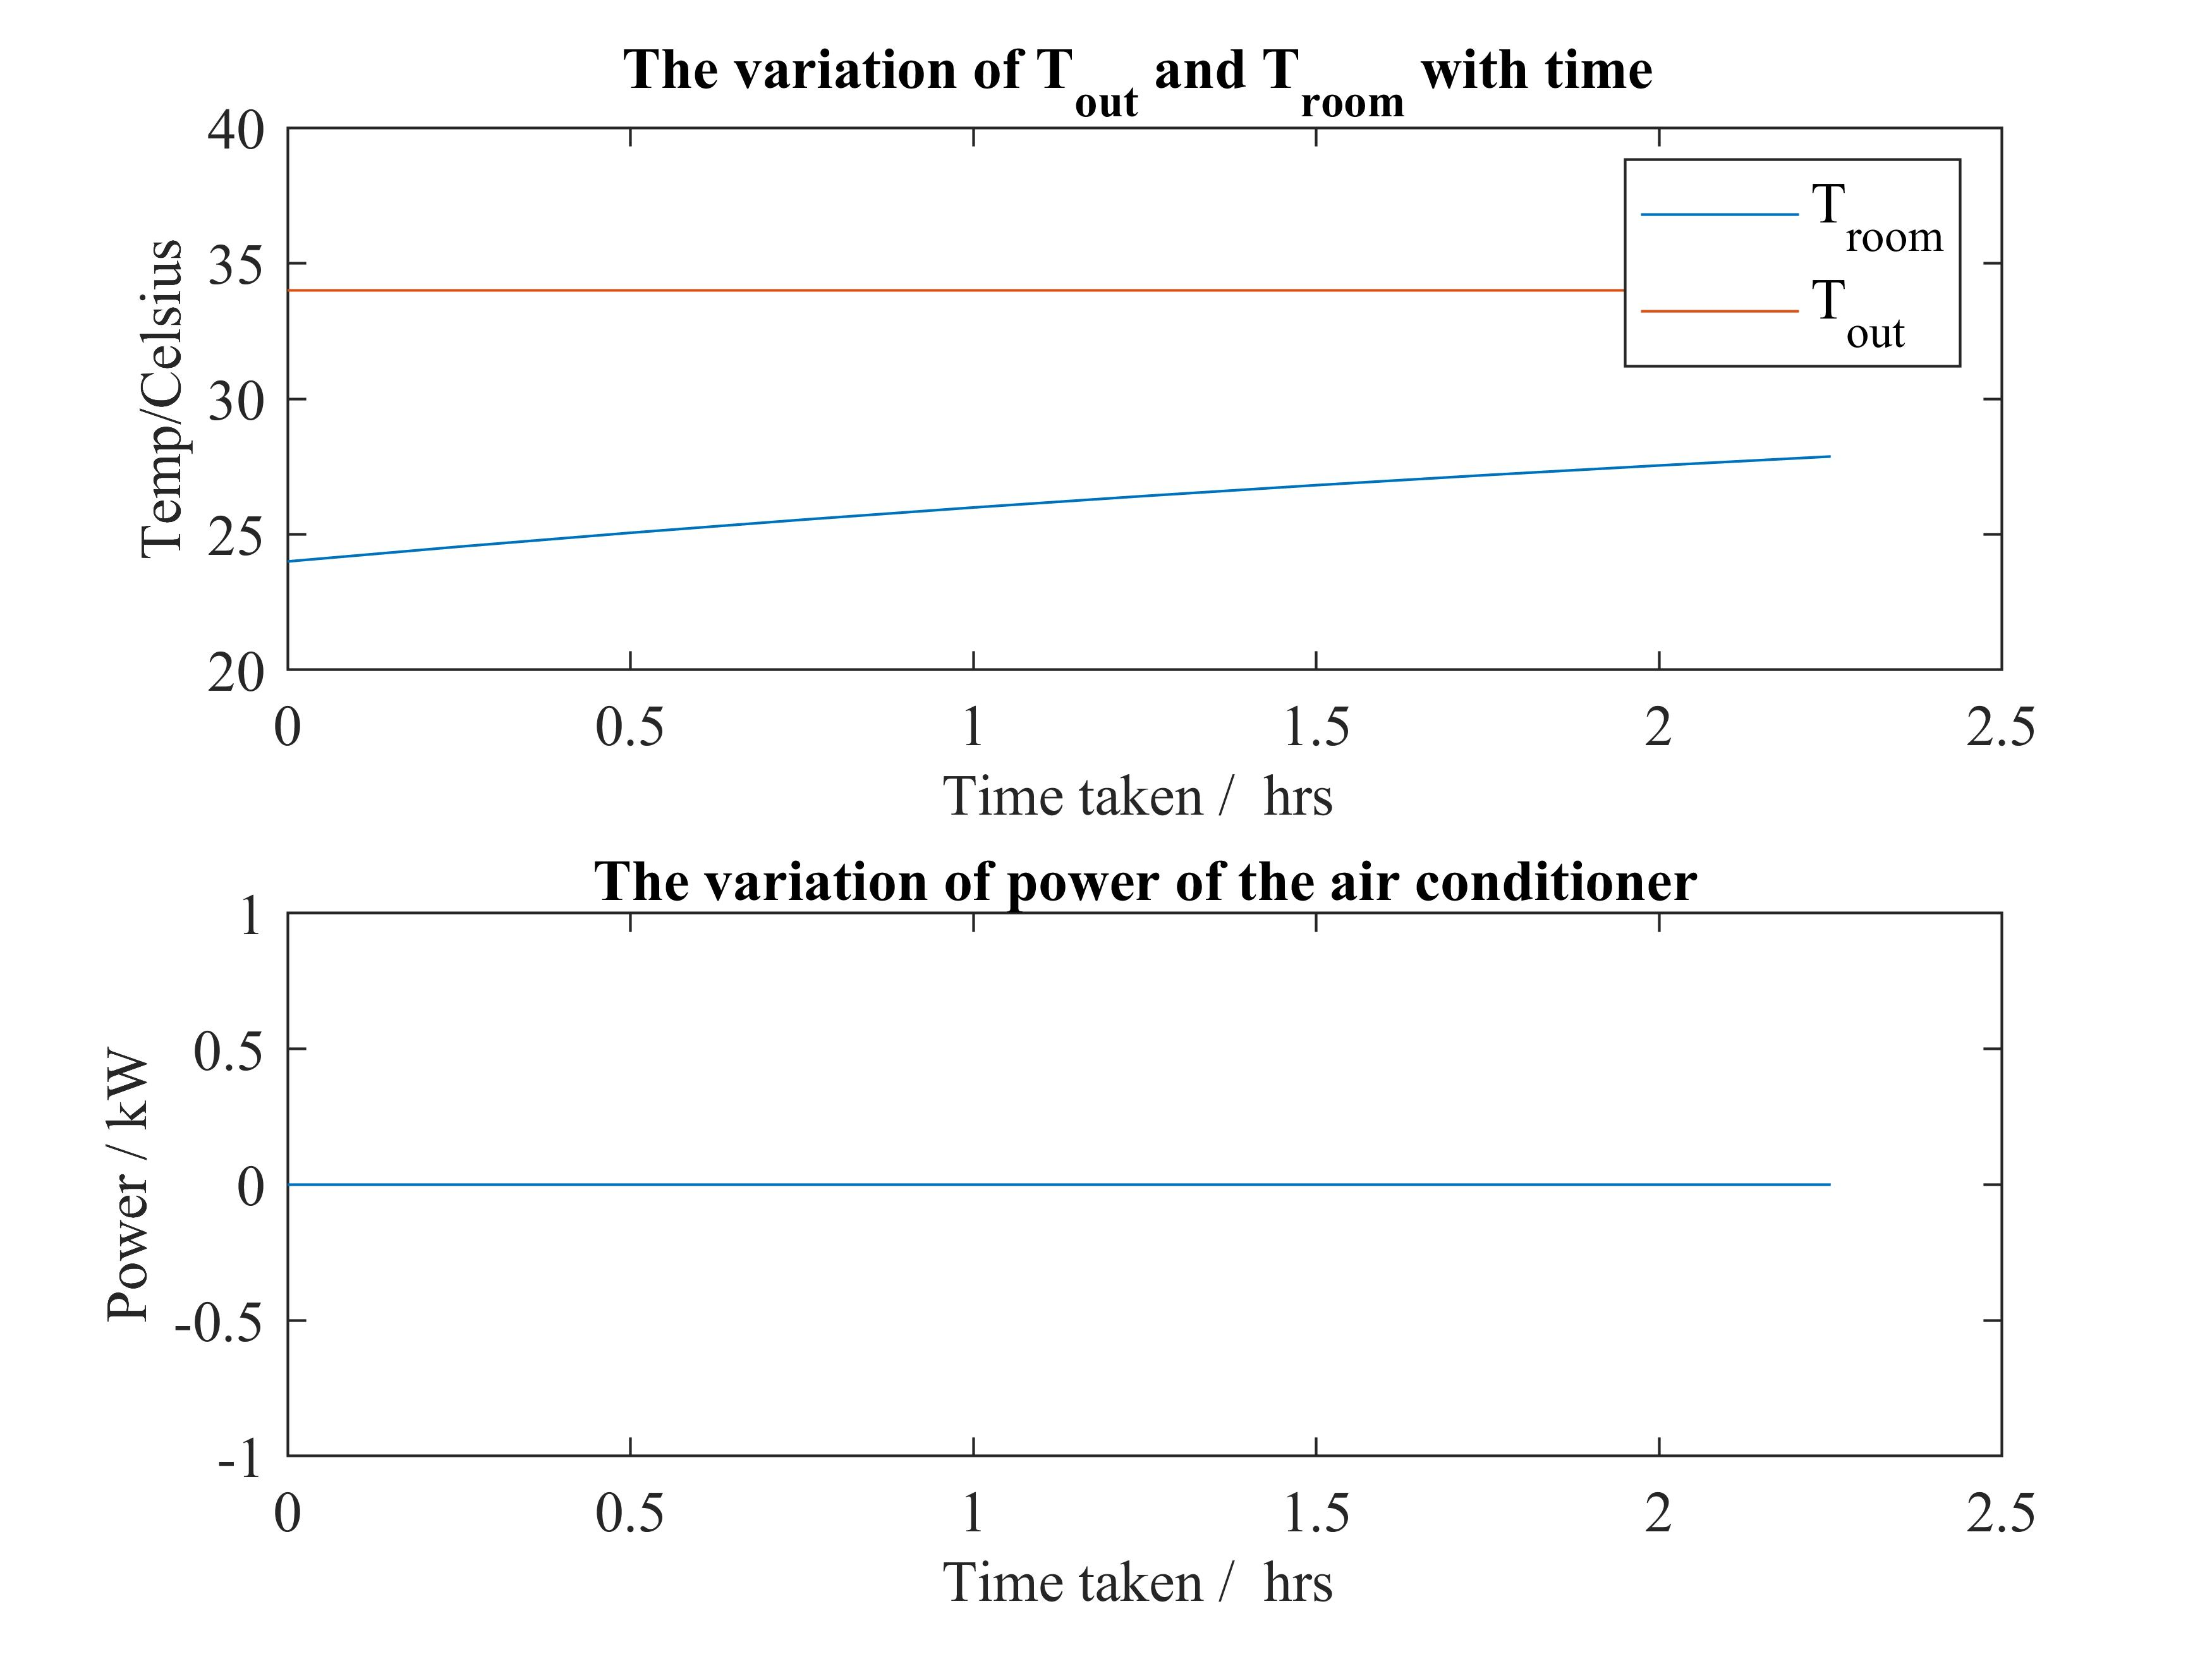
\includegraphics[width=13cm]{images/power_at_zero.jpg}
    \caption{The variation of room temperature with time}
    \label{fig:zeropower}
\end{figure}

According to figure \ref{fig:zeropower}, it is obvious that it takes a very long time for indoor temperature to reach the outdoor temperature when the air conditioner is switched off.\\

It is further elaborated with the following figure,

\pagebreak
\begin{figure}[htb]
    \centering
    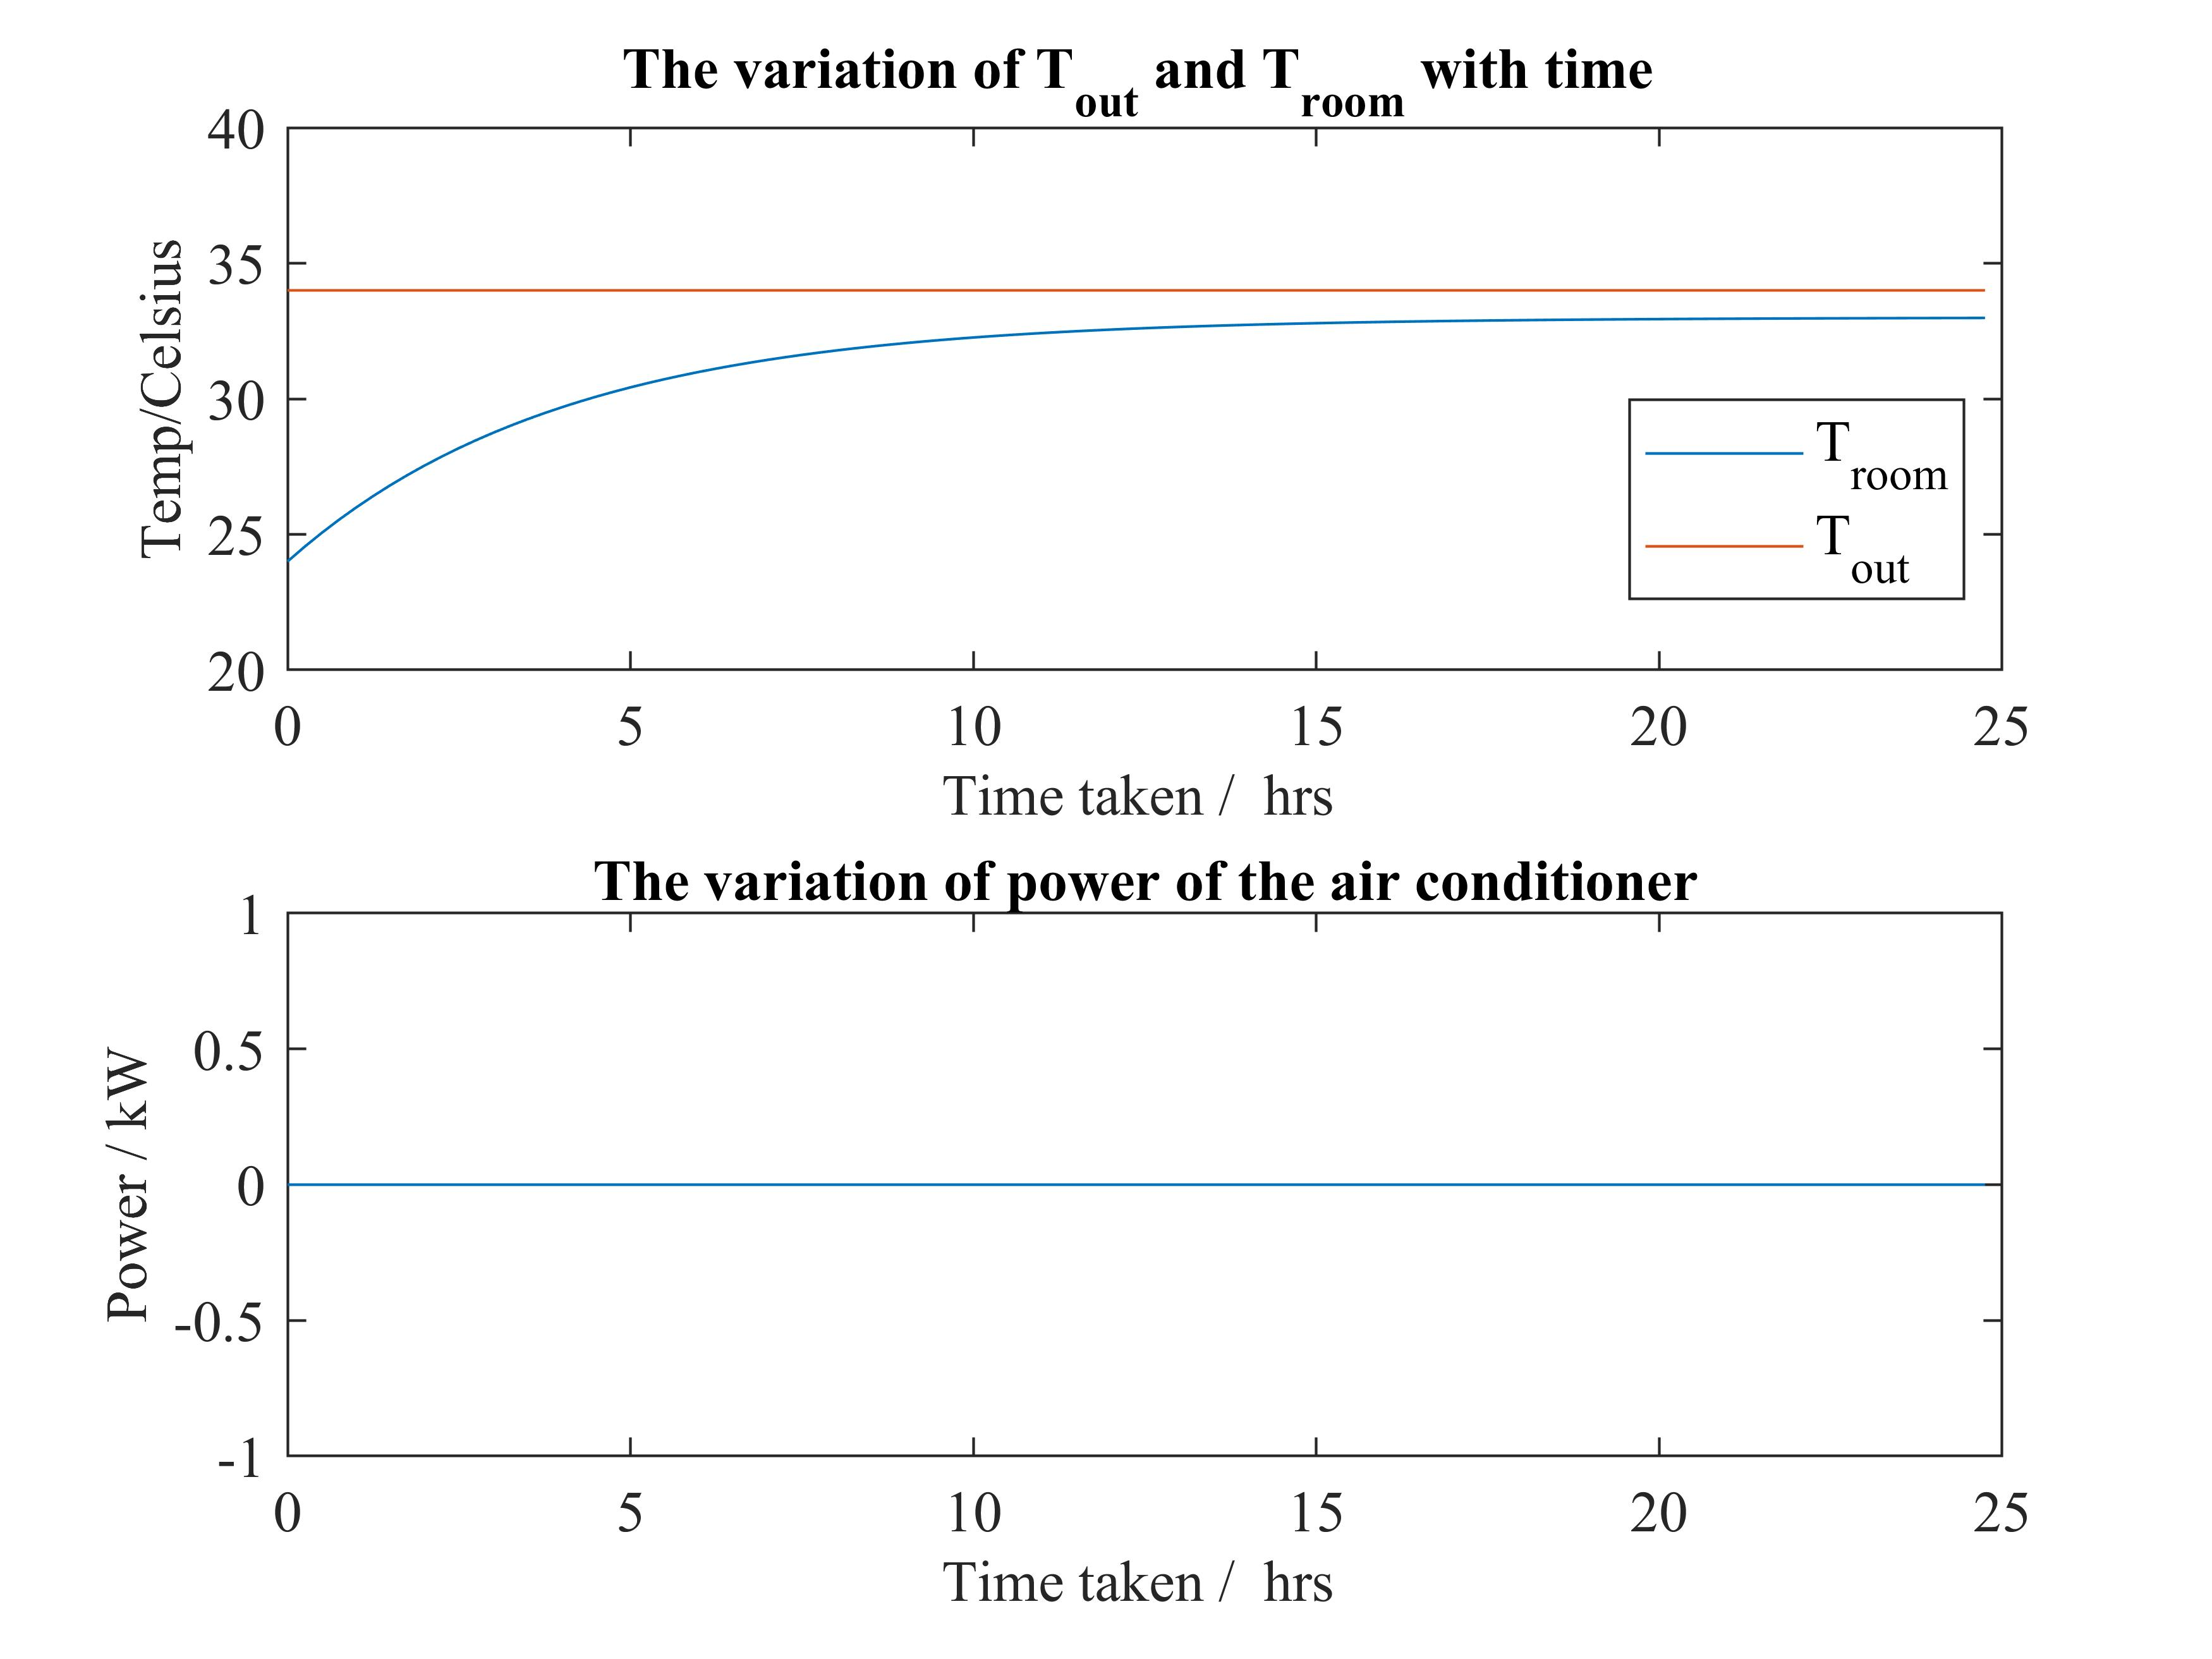
\includegraphics[width=13cm]{images/power_at_zero_long_iterations.jpg}
    \caption{The variation of room temperature with time for a longer period of time}
    \label{fig:zeropower_with_log_iterations}
\end{figure}
\end{itemize}


\subsection*{Considering situation 2,}

Electrical power output of the air conditioner was varied in different discrete levels to observe the how it affects the indoor temperature.

\begin{figure}[h!]
    \centering
    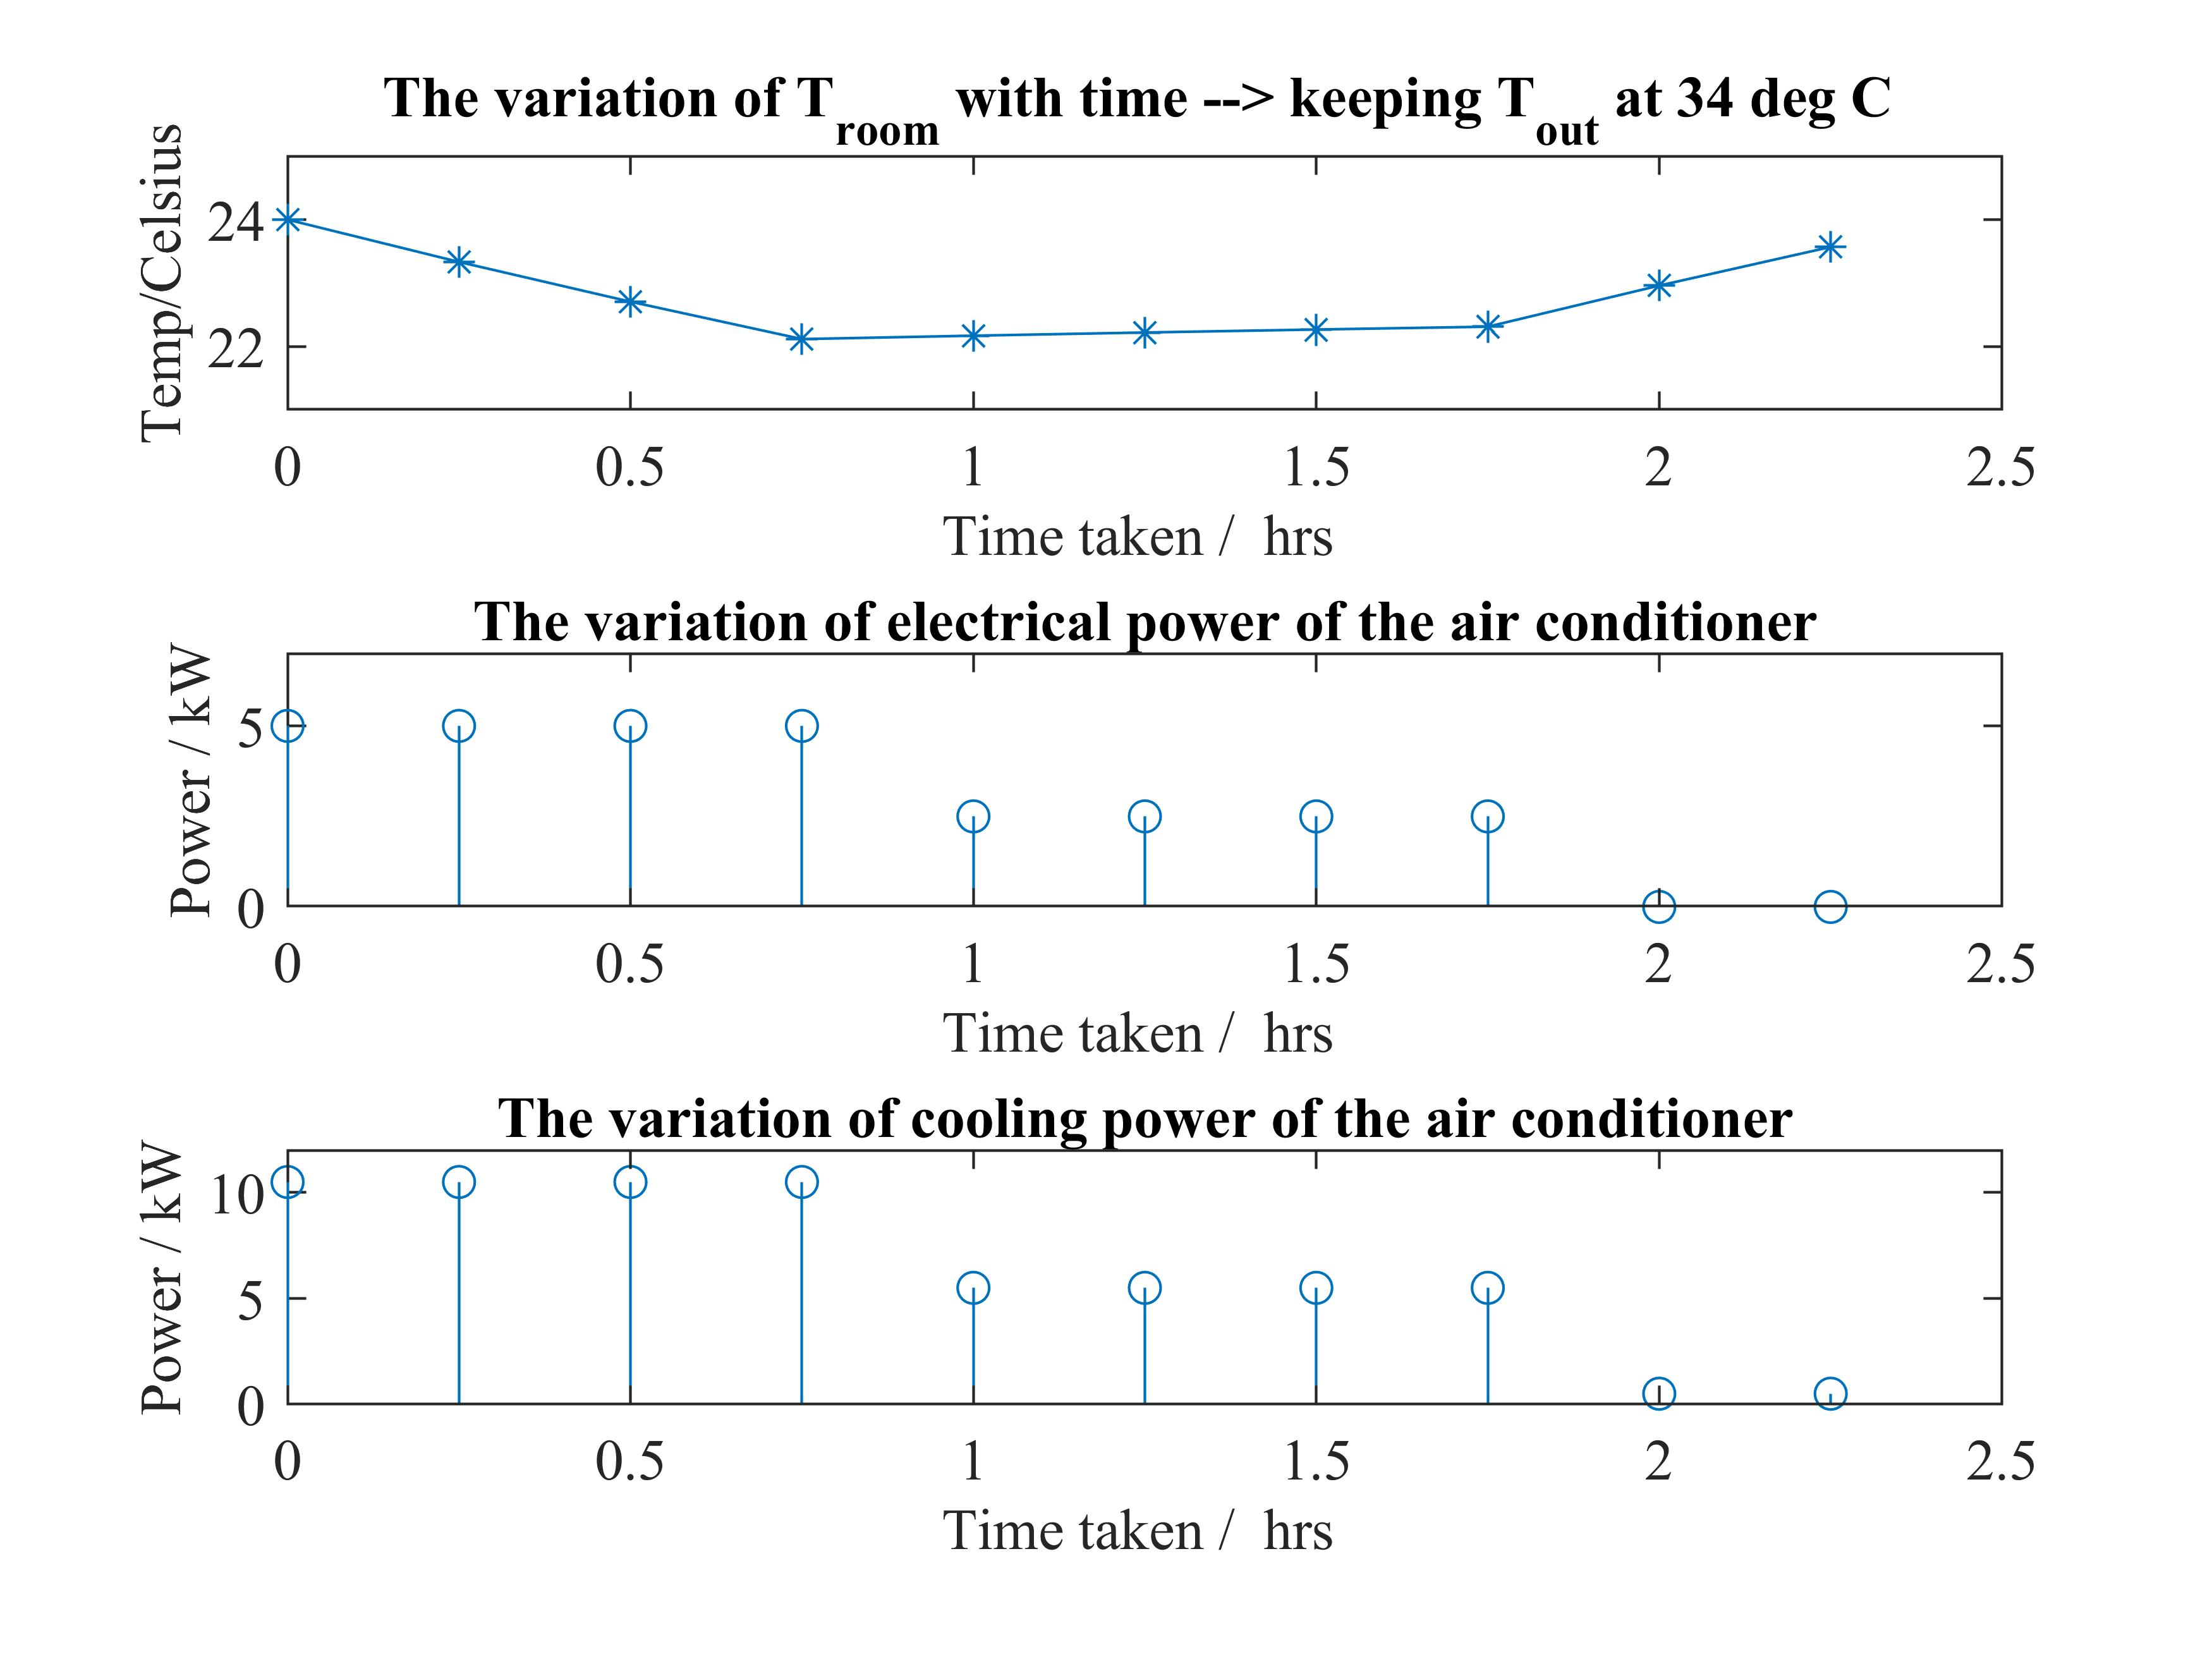
\includegraphics[width=13cm]{images/for_varying_power_levels_with_Q.jpg}
    \caption{The variation of indoor temperature for different power levels of the air conditioner}
    \label{fig:my_label}
\end{figure}

The initial temperature was 24\degree C. Until 45 mins, the air conditioner operated at the rated power of 5 kW. So the temperature dropped. Thereafter the air conditioner kept operating at 2.5 kW (half power) for 1 hour where the temperature slowly increased. Finally the air conditioner was switched off during which the temperature increased rapidly.\\

Another important point to consider here is that although P was zero for the last two time steps, the cooling power was not exactly zero.\\


\subsection*{Considering situation 3,}

In scenario 3, it was required to identify the cooling power as well the electrical power that should be supplied to keep the indoor temperature operating at 24\degree C while the outdoor temperature remains at 34\degree C.\\

With equation \eqref{eq:discretised_ETP_model},

\begin{equation}
    T_{t+1}^{in} = T_{t}^{in} = T_{t}^{out} - Q\cdot R
\end{equation}

\begin{figure}[h!]
    \centering
    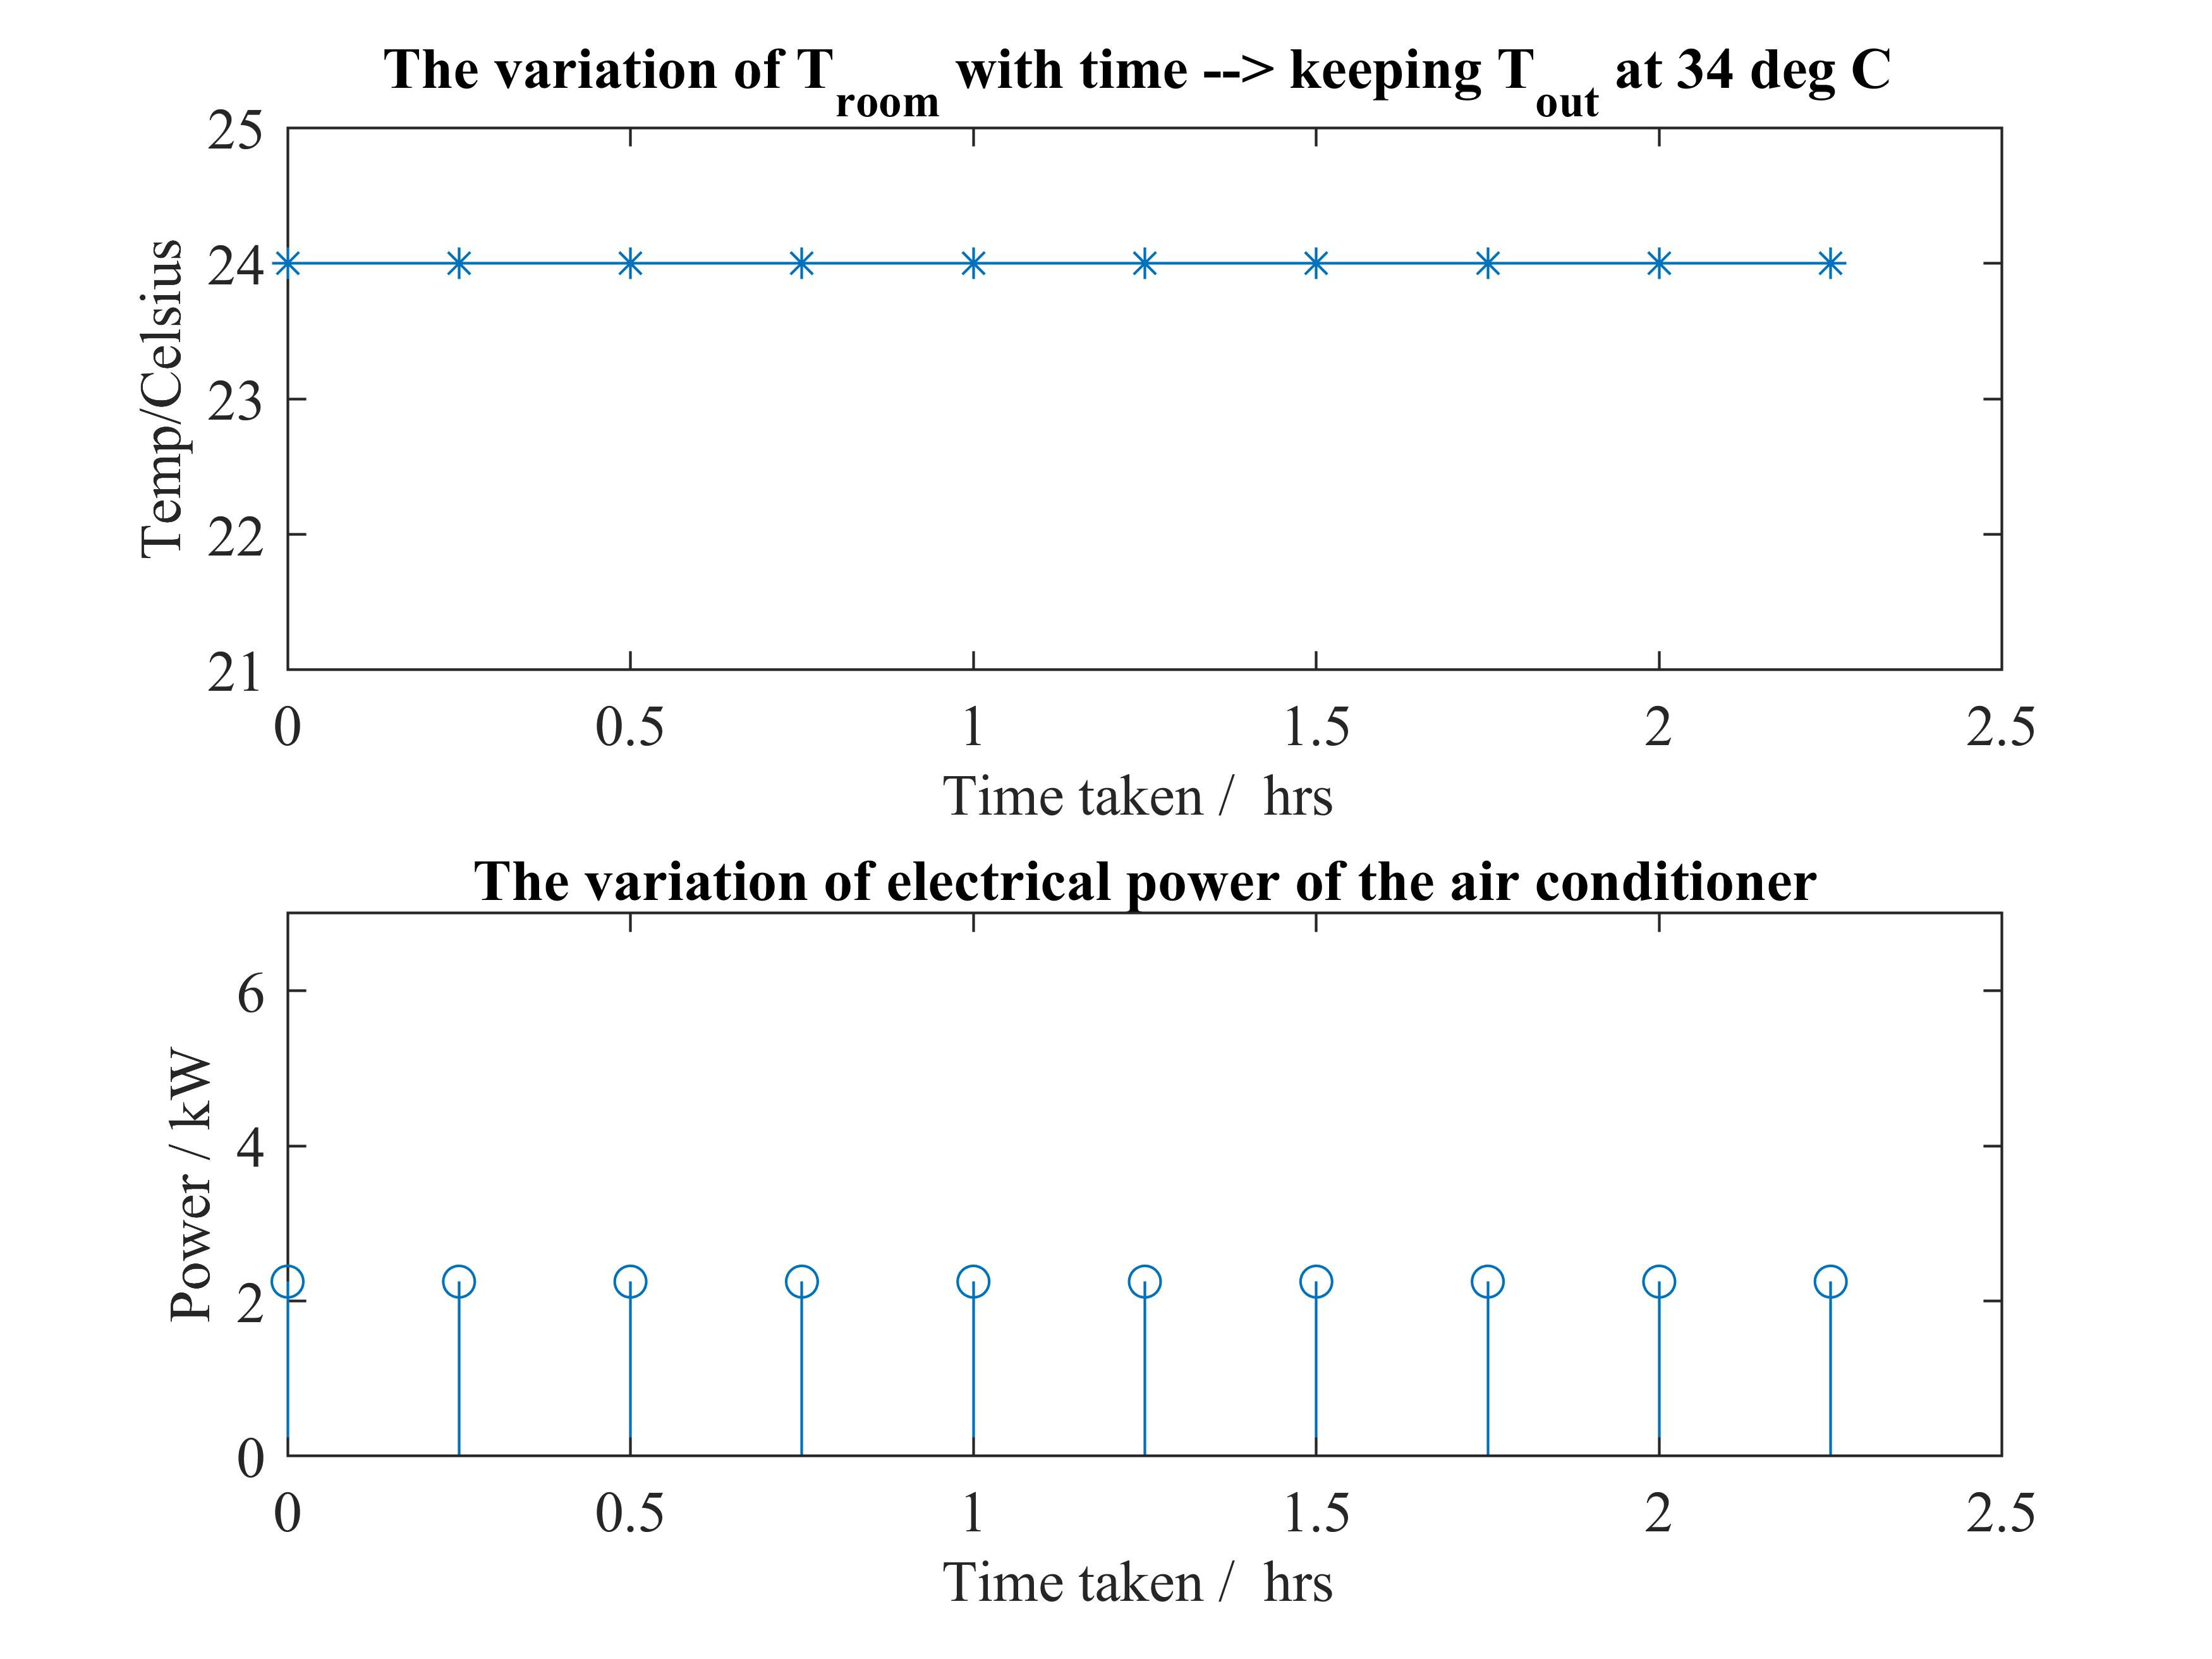
\includegraphics[width=13cm]{images/constant_P_and_T.jpg}
    \caption{The variation of indoor temperature with electrical power}
    \label{fig:constant_P}
\end{figure}

As long as the cooling power Q = 5 kW and P = 2.25 kW, the indoor temperature which was initially at 24\degree C remains constant.

\subsection*{Considering situation 4,}

The lower limit and the upper limit of the set point temperature was assumed to be 22\degree C and 27\degree C respectively. Thereafter the behaviour of the room temperature within the predefined limits were studied for the case where the demand response occured when the room temperature was 24\degree C.

\pagebreak

\begin{figure}[htb!]
    \centering
    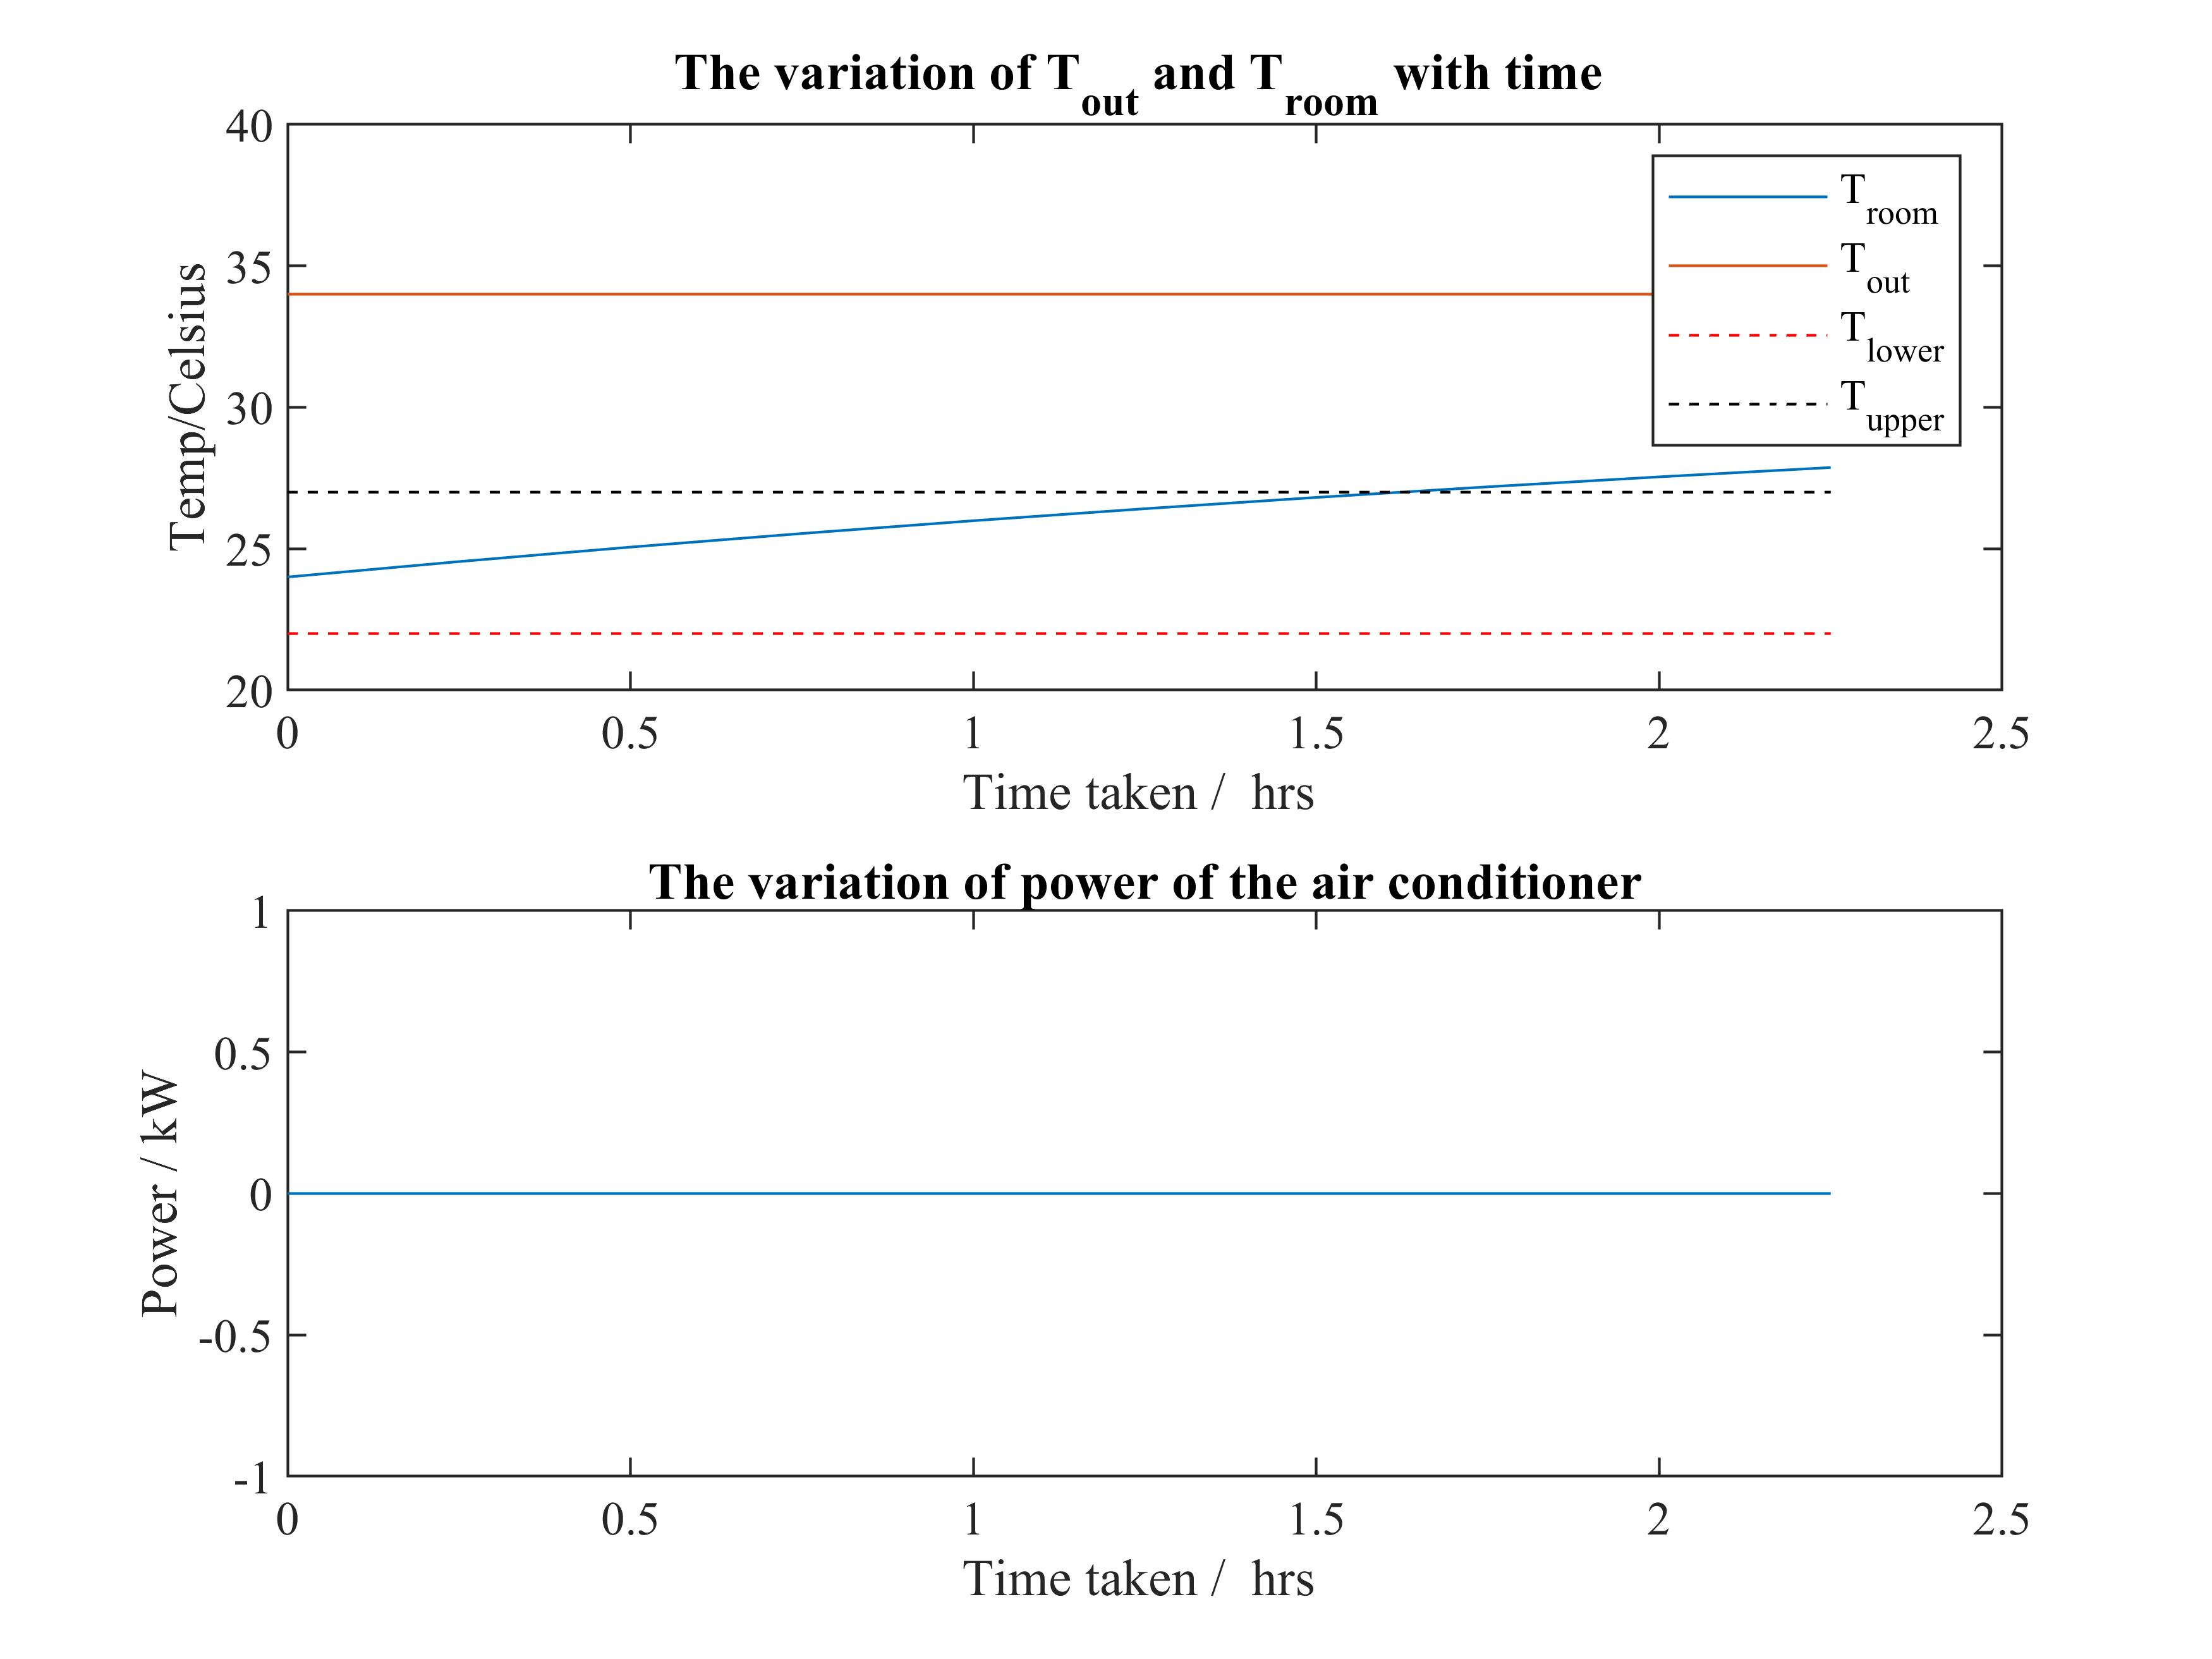
\includegraphics[width=14cm]{images/power_at_zero_with_set_limits.jpg}
    \caption{Variation of room temperature during the demand response event}
    \label{fig:with_set_limits}
\end{figure}

\textcolor{red}{From figure \ref{fig:with_set_limits} it was observed that the room temperature violates the upper level of the set point temperature only after 1.5 hrs once the air conditioner is completely switched off.} \\

\textcolor{red}{Hence there arises the question "Why do we need to control the power at discrete levels instead of switching off the device completely during the demand response event because switching off the device will not cause harm at all until 1.5 hrs from the beginning of the event."}



\bibliographystyle{ieeetr}
\bibliography{references}


\end{document}